\chapter{Application (practical)}
This part will discuss our model's practical implementation and programming tools. The practical implementation should also be divided into three parts: pre-processing, processing, and post-processing, which correspond to the theoretical design in the last chapter. \cite{t2m_1} used \textit{Java} as the programming tool in their work, yet their work was published 12 years ago, and during this period, a lot of tools in Artificial intelligence emerged. Thus, we decided to use \textit{Python} as the programming language with the \textit{Spacy}\footnote{https://spacy.io}, which is an open-source library especially for performing natural language processing tasks. The reason why we choose this library is that it has a good accuracy of 90.53\% on average. Besides, it also has a relatively good execution time \cite{complement_1}.

First, the input file should be the regulatory documents stored in raw text form, e.g., company policies, laws, etc. According to the theoretical design, the input file should be broken into sentences and tagged with correct grammatical labels. \textit{Spacy} integrates these functions in its core and will make the document pre-processing efficient. The processed sentences are stored in a python \textit{doc} class, which contains every word in the sentence stored in an object. Such an object possesses all the features of the word, such as the word's tokenization, part of speech tagging, sentence recognition, and so on \cite{complement_1}. Several works \cite{t2m_1} \cite{t2m_2} \cite{t2m_4} also suggest that the \textit{Stanford parser} is a widely adopted part of speech tagging tool with good recognition accuracy and a wide range of \textit{Stanford Dependencies}, which represents the grammatical relationships between words. 

The information stored in the python \textit{doc} class will be used for the main procedure of text-level analysis. \cite{literature_review_4} \cite{t2m_1} address the anaphora resolution problem using the \textit{WordNet} and \textit{FrameNet}, which are a lexical database of English used to perform semantic analysis. To detect conditional markers, a list of signal words can be predefined. \cite{complement_1} summarized the list of XOR and AND gateways, while \cite{t2m_1} gives four lists: ConditionIndicators, ParallelIndicators, ExceptionIndicators, and SequenceIndicators, which accordingly represents the exclusive gateway, parallel gateway, error intermediate events and continuation of a branch of a gateway. \cite{t2m_1} also gives a good illustration of how to generate the flows between activities, which represent their interactions. 

\begin{figure}[h]
    \centering
    \caption{Logical partition of approach's functions}
    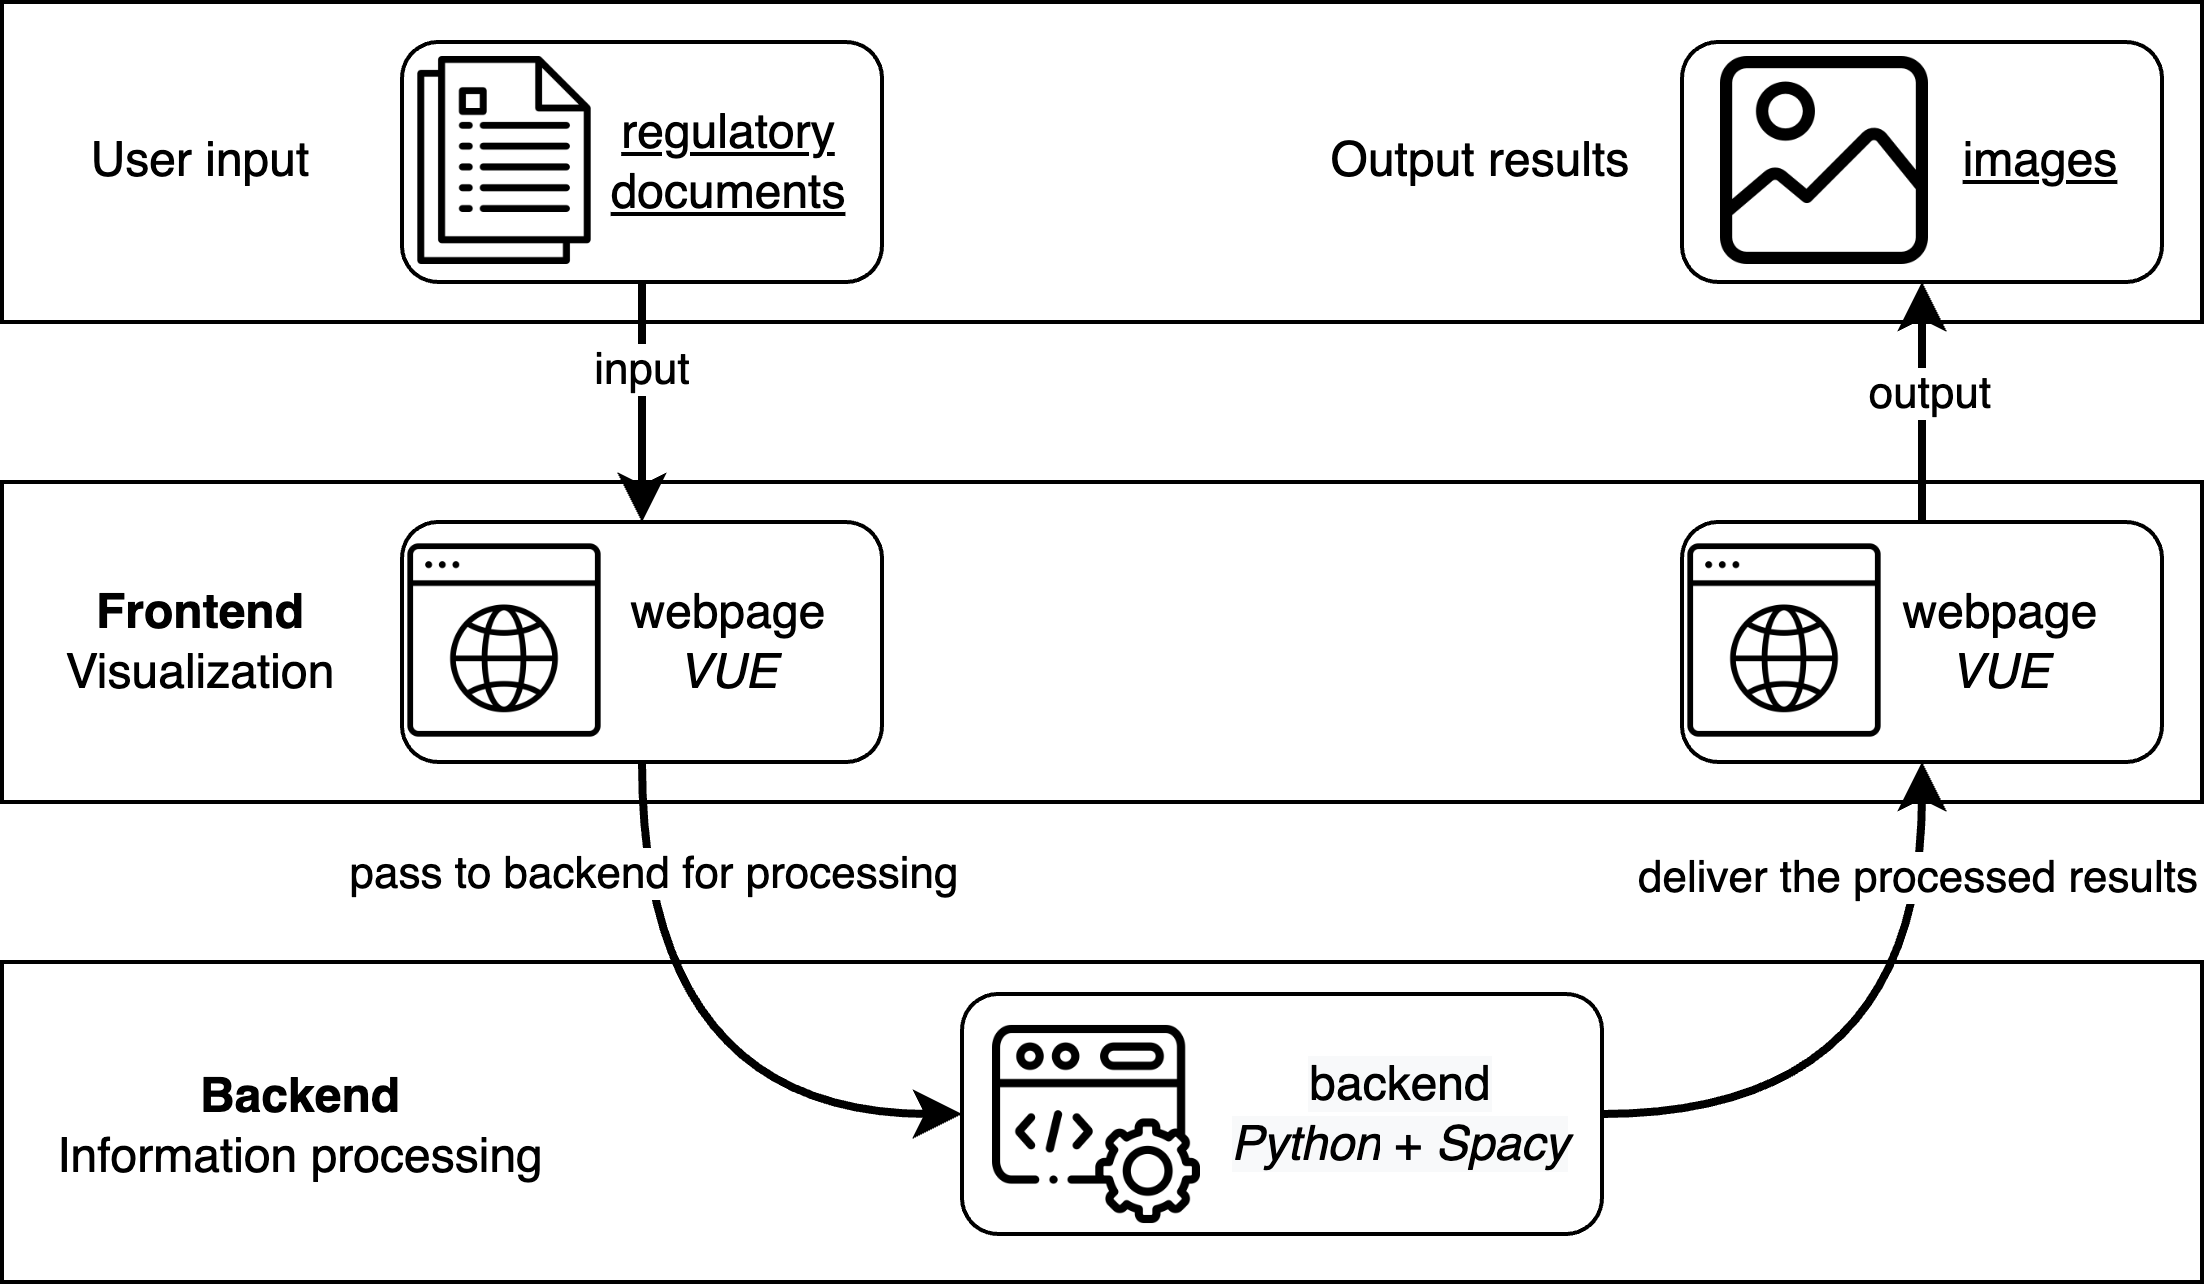
\includegraphics[width=0.9\textwidth]{tum-resources/images/Application_frontbackend.png}
    \floatfoot{Overview of the practical implementation of the proposed approach}
\end{figure}

Finally, the identified business activities connected using flows can be used for the generation of BPMN models. We can create a list of rules to convert the flows into the process models. \cite{literature_review_1} also suggests a list of BPMN modeling tools that can be leveraged to generate process models, which we will look further into. As mentioned, a web-based frontend should be created to increase the usability of our conversion model. The plan is to use \textit{Vue} as the framework to create such a website. The website should be able to have a text input area where the user can enter the regulatory text. Then the text will be delivered to our \textit{Python} backend and processed. The final results will be sent back to the website and displayed in the form of an image. 


